\clearpage
\phantomsection
\section*{四、CEC 下的资源自适应的模型切分部署方法}
\addcontentsline{toc}{section}{四、CEC 下的资源自适应的模型切分部署方法}

大语言模型推理在 CEC 场景下面临的首要问题，不只是单个模型能否放入某个设备，而是同一次推理中的模型结构、计算阶段和运行时状态能否被合理分布到端侧、接入边缘、区域边缘和云端。端侧设备靠近用户并具有隐私优势，但算力、内存、功耗和散热约束严格；边缘节点提供近用户算力，却常常呈现资源碎片化、设备异构和负载波动；云端算力充足，但网络往返、带宽消耗和数据出域风险会进入端到端服务路径。模型切分部署的价值，正是在这些资源边界之间重新组织一次推理，使大模型不再被单个节点的容量和位置限制。Petals 说明大模型可以通过协作式 block 放置突破单节点容量限制 \cite{borzunov2023petals}，HexGen 说明异构 GPU 和异构网络会改变生成式推理的并行策略 \cite{jiang2023hexgen}，FlexGen 则从单 GPU 场景展示权重、activation 和 KV Cache 的分层放置对吞吐的影响 \cite{sheng2023flexgen}。这些工作共同表明，LLM 推理的部署瓶颈通常同时来自模型权重、activation、KV Cache、互联带宽和运行时调度，而不是单一计算瓶颈。
与一般服务路由不同，模型切分部署关心的是推理内部的执行结构是否发生变化。仅在多个完整模型或完整服务实例之间选择执行路径的方法，本质上属于服务路径选择或负载均衡；它可能影响时延和成本，但没有切分模型本体，也没有改变一次推理中计算、状态或生成职责的组织方式。因此，本章只讨论会改变模型执行拓扑、层内并行方式、推理阶段边界或 token 生成职责分工的方法。这样的边界可以避免把“请求发到哪里”和“模型如何被拆开执行”混为一谈，也便于比较不同方法真正改变的系统对象。
本章将 request-level routing 排除在模型切分部署之外，是为了保持分类口径一致；若请求路由同时触发模型段迁移、阶段迁移或 expert 组件迁移，则其模型执行结构变化部分仍可纳入本章讨论。
本文按 primary optimization object 将相关方法划分为五类：
\begin{enumerate}
\item \textbf{Layer-wise / Vertical Partitioning}：切的是 Transformer 深度方向，决定 layer、block 或 model shard 放在哪些节点上执行。
\item \textbf{Tensor / Operator-level Partitioning}：切的是同一层内部的计算单元，决定 attention head、MLP 矩阵、tensor shard 或 communication primitive 如何并行。
\item \textbf{Expert / Component-level Partitioning}：切的是 MoE expert 等模型组件，决定哪些 expert 常驻、换入、映射或跨层级放置。
\item \textbf{Inference Phase Partitioning}：切的是 prefill、decode、verification、download 等执行阶段，利用不同阶段的资源画像差异。
\item \textbf{Semantic / Token-level Partitioning}：切的是生成过程本身，决定 draft、verify、semantic segment、token-wise partition 等语义单元如何协作。
\end{enumerate}

这五类方法不是严格互斥的。Jupiter 同时涉及边缘协作执行和 prefill/decode 阶段组织 \cite{ye2025jupiter}；TensAllo 同时包含设备选择、模型部署和张量并行 \cite{zhang2025tensallo}；Mooncake 以 prefill/decode 解耦为主，但其收益依赖分布式 KV Cache \cite{qin2025mooncake}；SwapMoE 则更接近专家级动态驻留与换入 \cite{kong2024swapmoe}。本文按主要优化对象归类，交叉关系在总览表中保留。这个口径的目的不是把每篇工作强行放进唯一格子，而是让读者能看清：某个方法到底是在切模型深度、切层内计算、切专家组件、切执行阶段，还是切生成语义。

表中“切分类型”表示论文中最接近本章 taxonomy 的主优化对象，不等价于论文全部贡献。例如 Mooncake 的核心贡献包含 KVCache-centric 架构，本章将其放入阶段切分，是因为其服务路径首先建立在 prefill/decode disaggregation 之上 \cite{qin2025mooncake}。

表~\ref{tab:cec-model-partition-overview} 汇总了本章五类模型切分部署方法的代表工作、发表位置、切分类型、优化目标与加速机制；图~\ref{fig:cec-model-partition-taxonomy} 进一步以树状结构展示五类方法、主要切分对象和代表工作之间的对应关系。

\begingroup
\scriptsize
\setlength{\tabcolsep}{1.4pt}
\renewcommand{\arraystretch}{1.35}
\emergencystretch=2em
\begin{longtable}{@{}>{\raggedright\arraybackslash\hspace{0pt}}p{0.035\textwidth} >{\raggedright\arraybackslash\hspace{0pt}}p{0.205\textwidth} >{\raggedright\arraybackslash\hspace{0pt}}p{0.085\textwidth} >{\raggedright\arraybackslash\hspace{0pt}}p{0.105\textwidth} >{\raggedright\arraybackslash\hspace{0pt}}p{0.105\textwidth} >{\raggedright\arraybackslash\hspace{0pt}}p{0.155\textwidth} >{\raggedright\arraybackslash\hspace{0pt}}p{0.270\textwidth}@{}}
\caption{\textbf{CEC 下资源自适应模型切分部署方法相关工作}}
\label{tab:cec-model-partition-overview}\\
\toprule
\textbf{序号} & \textbf{System / Framework} & \textbf{Venue / Year} & \textbf{切分类型} & \textbf{Objectives} & \textbf{Optimization Technology} & \textbf{加速机制 / 方法核心} \\
\midrule
1 & Jupiter: Fast and Resource-Efficient Collaborative Inference of Generative LLMs on Edge Devices \cite{ye2025jupiter} & IEEE INFOCOM 2025 & 层级切分 / 推理阶段切分 & prefill/decode 协同执行 & intra-sequence pipeline parallelism; outline-based pipeline parallel decoding; speculative decoding & Prefill 阶段用序列内流水线并行分摊长 prompt 计算；decode 阶段用 outline-based pipeline parallel decoding 和 speculative decoding 减少自回归串行步数与流水线气泡 \\
\tabrowrule
2 & TensAllo: Adaptive Deployment of LLMs on Resource-Constrained Heterogeneous Edge Devices \cite{zhang2025tensallo} & IEEE INFOCOM 2025 & 层级切分 / 张量切分 & 在资源受限异构边缘设备上部署 LLM & adaptive device selection; tensor allocation; tensor parallelism; quantization & 通过设备选择和 tensor allocation 把计算分配到更合适的异构设备；再用量化降低内存占用，使更多 tensor shard 能留在边缘设备上执行 \\
\tabrowrule
3 & EdgeShard: Efficient LLM Inference via Collaborative Edge Computing \cite{zhang2024edgeshard} & IEEE IoT Journal 2025 & 层级切分 / 垂直切分 & 模型分片放置 & model shard placement; joint device selection; dynamic programming & 将 LLM 切成 model shards，并联合选择设备和 shard placement；动态规划寻找计算时延、传输代价和 pipeline 吞吐之间更优的放置方案 \\
\tabrowrule
4 & Petals: Collaborative Inference and Fine-tuning of Large Models \cite{borzunov2023petals} & ACL 2023 Demo & 层级切分 / 垂直切分 & 将大模型 block 分布到多个参与节点 & decentralized layer/block placement; pipeline across volunteered servers & 把 Transformer block 分散存放在志愿节点 GPU 上，客户端按 pipeline 顺序调用连续 block，避免本地 RAM/SSD offloading 反复搬运完整权重 \\
\tabrowrule
5 & HexGen: Generative Inference of Large Language Model over Heterogeneous Environment \cite{jiang2023hexgen} & ICML 2024 & 层级切分 / 张量切分 & 在异构 GPU 和异构网络上组织生成式推理 & asymmetric tensor parallelism; pipeline parallelism; constrained scheduling & 同时允许 pipeline stage 和 tensor parallel degree 非对称配置，让快慢 GPU、异构链路承担不同计算份额，而不是强制所有 stage 使用同构并行度 \\
\tabrowrule
6 & Resource-Efficient Collaborative Edge Transformer Inference With Hybrid Model Parallelism \cite{ye2025resource} & IEEE TMC 2025 & 层级切分 / 张量切分 & 混合并行协同推理 & hybrid model parallelism; heterogeneity- and memory-aware planning; communication overlap & 用 hybrid model parallelism 结合 layer/pipeline 与 tensor 并行；通过 ReduceScatter/AllGather 替代部分 AllReduce，并用通信-计算重叠降低边缘弱链路上的同步等待 \\
\tabrowrule
7 & Co-Designing Transformer Architectures for Distributed Inference With Low Communication \cite{du2024co} & IEEE TPDS 2025 & 张量/算子级切分 & 降低分布式 Transformer 推理通信 & low-communication architecture co-design; block parallelism; two-phase planning & 通过把原 Transformer layer 重构为多个 decoupled sub-block 暴露 block parallelism，减少层内强依赖和 all-reduce 次数，再用离线权重放置与在线并行规划选择低通信执行路径 \\
\tabrowrule
8 & FlexGen: High-throughput Generative Inference of Large Language Models with a Single GPU \cite{sheng2023flexgen} & ICML 2023 & 张量/算子级切分 & 在单 GPU 资源受限环境中服务大模型 & tensor/KV/activation placement; GPU-CPU-disk offloading; linear programming & 把权重、activation 和 KV cache 在 GPU、CPU、磁盘之间分层放置，用线性规划选择 offloading 和访问模式，并结合压缩扩大 batch size 与吞吐 \\
\tabrowrule
9 & E2LLM: Structure-Guided Efficient Inference for LLMs in Distributed Edge-IoT Environments \cite{feng20262} & IEEE TMC 2026 & 推理阶段切分 / 语义级协同切分 & 边缘结构规划与 IoT 并行解码 & structure-guided planning; static-dynamic KV cache partitioning; distributed decoding & 边缘节点负责结构规划和 segment-specific KV 生成，IoT 设备并行执行轻量 decoding；静态/动态 KV 分离减少重复传输，并用 response skeleton 保持片段语义一致 \\
\tabrowrule
10 & FlexPipe: Adapting Dynamic LLM Serving Through Inflight Pipeline Refactoring in Fragmented Serverless Clusters \cite{lin2026flexpipe} & EuroSys 2026 & 层级切分 / 垂直切分 & 运行时 pipeline stage 重构 & fine-grained model partitioning; inflight pipeline refactoring; topology-aware allocation & 将模型预切成细粒度 stage，并在请求执行中动态调整 pipeline granularity；通过一致的 cache transition 和拓扑感知资源分配适配碎片化 GPU \\
\tabrowrule
11 & DistServe: Disaggregating Prefill and Decoding for Goodput-optimized LLM Serving \cite{zhong2024distserve} & OSDI 2024 & 推理阶段切分 & prefill/decode 物理解耦 & phase-specific workers; phase-aware parallelism; KV transfer & 将 compute-heavy prefill 与 memory/latency-sensitive decode 分配给不同 worker pool；分别选择并行度和 batch 策略，再通过 KV transfer 连接两阶段 \\
\tabrowrule
12 & Splitwise: Efficient Generative LLM Inference Using Phase Splitting \cite{patel2024splitwise} & ISCA 2024 & 推理阶段切分 & prompt/token 阶段分离 & prompt pool; token pool; hardware matching; overlapped KV transfer & 将 prompt computation 和 token generation 拆到不同机器池，使两阶段匹配不同硬件；同时用 layer-wise/overlapped KV transfer 降低阶段切换的关键路径开销 \\
\tabrowrule
13 & Mooncake: Trading more storage for less computation -- A KVCache-centric architecture for serving LLM chatbot \cite{qin2025mooncake} & USENIX FAST 2025 & 推理阶段切分 & prefill/decode disaggregation & distributed KV cache; global scheduling; KVCache-centric architecture & 在 prefill/decode 解耦基础上构建分布式 KVCache，把 CPU、DRAM、SSD、NIC 作为共享状态层；调度器按 KV 复用、本地性和 SLO 选择 prefill/decode 实例 \\
\tabrowrule
14 & SLIDE: Simultaneous Model Downloading and Inference at the Wireless Network Edge \cite{qu2026slide} & IEEE TMC 2026 & 推理阶段切分 & 下载与推理重叠 & layer-wise download/inference overlap; bandwidth and compute allocation & 按 layer 递归依赖组织下载和执行：用户一边接收后续 layer，一边执行已下载 layer；联合优化带宽和计算分配以隐藏模型下载等待 \\
\tabrowrule
15 & EdgeLLM: Fast On-Device LLM Inference With Speculative Decoding \cite{xu2024edgellm} & IEEE TMC 2025 & 语义/token 级协同切分 & 减少端侧逐 token 解码开销 & on-device speculative decoding; branch navigation; self-adaptive fallback; compute-I/O pipeline & 小 draft LLM 常驻内存生成候选 token，大 target LLM 批量验证；用分支导航避免把算力浪费在低概率分支，并用 compute-I/O pipeline 隐藏大模型权重加载 \\
\tabrowrule
16 & SPIN: Accelerating Large Language Model Inference with Heterogeneous Speculative Models \cite{chen2025spin} & IEEE INFOCOM 2025 & 语义/token 级协同切分 & 异构草稿模型选择与验证流水线 & heterogeneous SSM selection; request decomposition; speculation/verification pipelining & 为不同难度请求选择合适的异构 speculative model；把长请求拆分以降低 verification batch padding，并流水化 speculation 与 verification 阶段 \\
\tabrowrule
17 & SpecInfer: Accelerating Large Language Model Serving with Tree-based Speculative Inference and Verification \cite{miao2024specinfer} & ASPLOS 2024 & 语义/token 级协同切分 & token tree 草稿与批量验证 & tree-based speculative inference; parallel verification & 多个小模型生成候选 token tree，目标 LLM 不再逐 token 增量生成，而是作为 verifier 一次并行校验多条候选路径，从而减少目标模型调用次数 \\
\tabrowrule
18 & SwapMoE: Serving Off-the-shelf MoE-based Large Language Models with Tunable Memory Budget \cite{kong2024swapmoe} & ACL 2024 & 专家/组件级切分 & 专家驻留可调 & virtual experts; expert swapping; tunable memory budget & 只把动态选择的重要专家作为 virtual experts 常驻主存，其余专家按需映射和换入，在不剪枝模型结构的情况下减少 MoE 推理内存占用和换入开销 \\
\tabrowrule
19 & Taming Latency-Memory Trade-Off in MoE-Based LLM Serving via Fine-Grained Expert Offloading \cite{yu2026taming} & EuroSys 2026 & 专家/组件级切分 & 细粒度 expert offloading & fine-grained expert offloading; latency-memory trade-off & 以 expert 为换入/卸载单元，在显存预算下决定哪些专家保留在 GPU、哪些下沉到主机或存储层，从而在显存节省和专家加载延迟之间折中 \\
\tabrowrule
20 & MoE-Infinity: Efficient MoE Inference on Personal Machines with Sparsity-Aware Expert Cache \cite{xue2024moe} & ICML 2025 & 专家/组件级切分 & 稀疏感知 expert cache & sparsity-aware expert cache; expert prefetching; memory hierarchy & 利用 MoE token 路由稀疏性和专家访问局部性，只缓存即将使用或高频专家，并通过预取和分层内存降低专家缺页造成的 decode 停顿 \\
\tabrowrule
21 & Pre-gated MoE: An Algorithm-System Co-Design for Fast and Scalable MoE Inference \cite{hwang2024pre} & ISCA 2024 & 专家/组件级切分 & 提前 expert routing 与系统协同 & pre-gating; expert scheduling; algorithm-system co-design & 在系统执行前更早获得 expert 选择信息，使 expert 加载、通信和调度可以提前安排，减少 MoE 推理中的路由等待和跨设备同步 \\
\tabrowrule
22 & EdgeMoE: Empowering Sparse Large Language Models on Mobile Devices \cite{yi2025edgemoe} & IEEE TMC 2025 & 专家/组件级切分 & 移动端稀疏 LLM 部署 & sparse MoE deployment; expert management; on-device inference & 面向移动设备资源约束管理 MoE expert 的驻留与执行，使稀疏大模型能够在端侧或近端资源上以可控内存开销运行 \\
\tabrowrule
23 & WDMoE: Wireless Distributed Mixture of Experts for Large Language Models \cite{xue2025wdmoe} & IEEE TWC 2025 & 专家/组件级切分 & 无线边缘分布式 MoE & wireless distributed experts; expert selection; bandwidth allocation & 将 gating/attention 和 experts 分布在基站与移动设备之间，根据 expert 权重、设备延迟和无线带宽联合选择专家与分配通信资源 \\
\tabrowrule
24 & P4LLM: Protecting Embedding Privacy against Model Inversion Attacks for EaaS LLM Serving via Token-wise Partition and Perturbation \cite{lu2026p4llm} & IEEE TMC 2026 & 语义/token 级协同切分 & token-wise partition + perturbation & insensitive token filtering; partitioning scheduler; hidden-state perturbation & 在用户侧按 token 切分 Transformer 执行，只对敏感 token 的 hidden state 做扰动并上传，非敏感 token 过滤或轻处理，从而减少扰动计算和传输负担 \\
\bottomrule
\end{longtable}
\endgroup

\begin{figure}[!htbp]
\centering
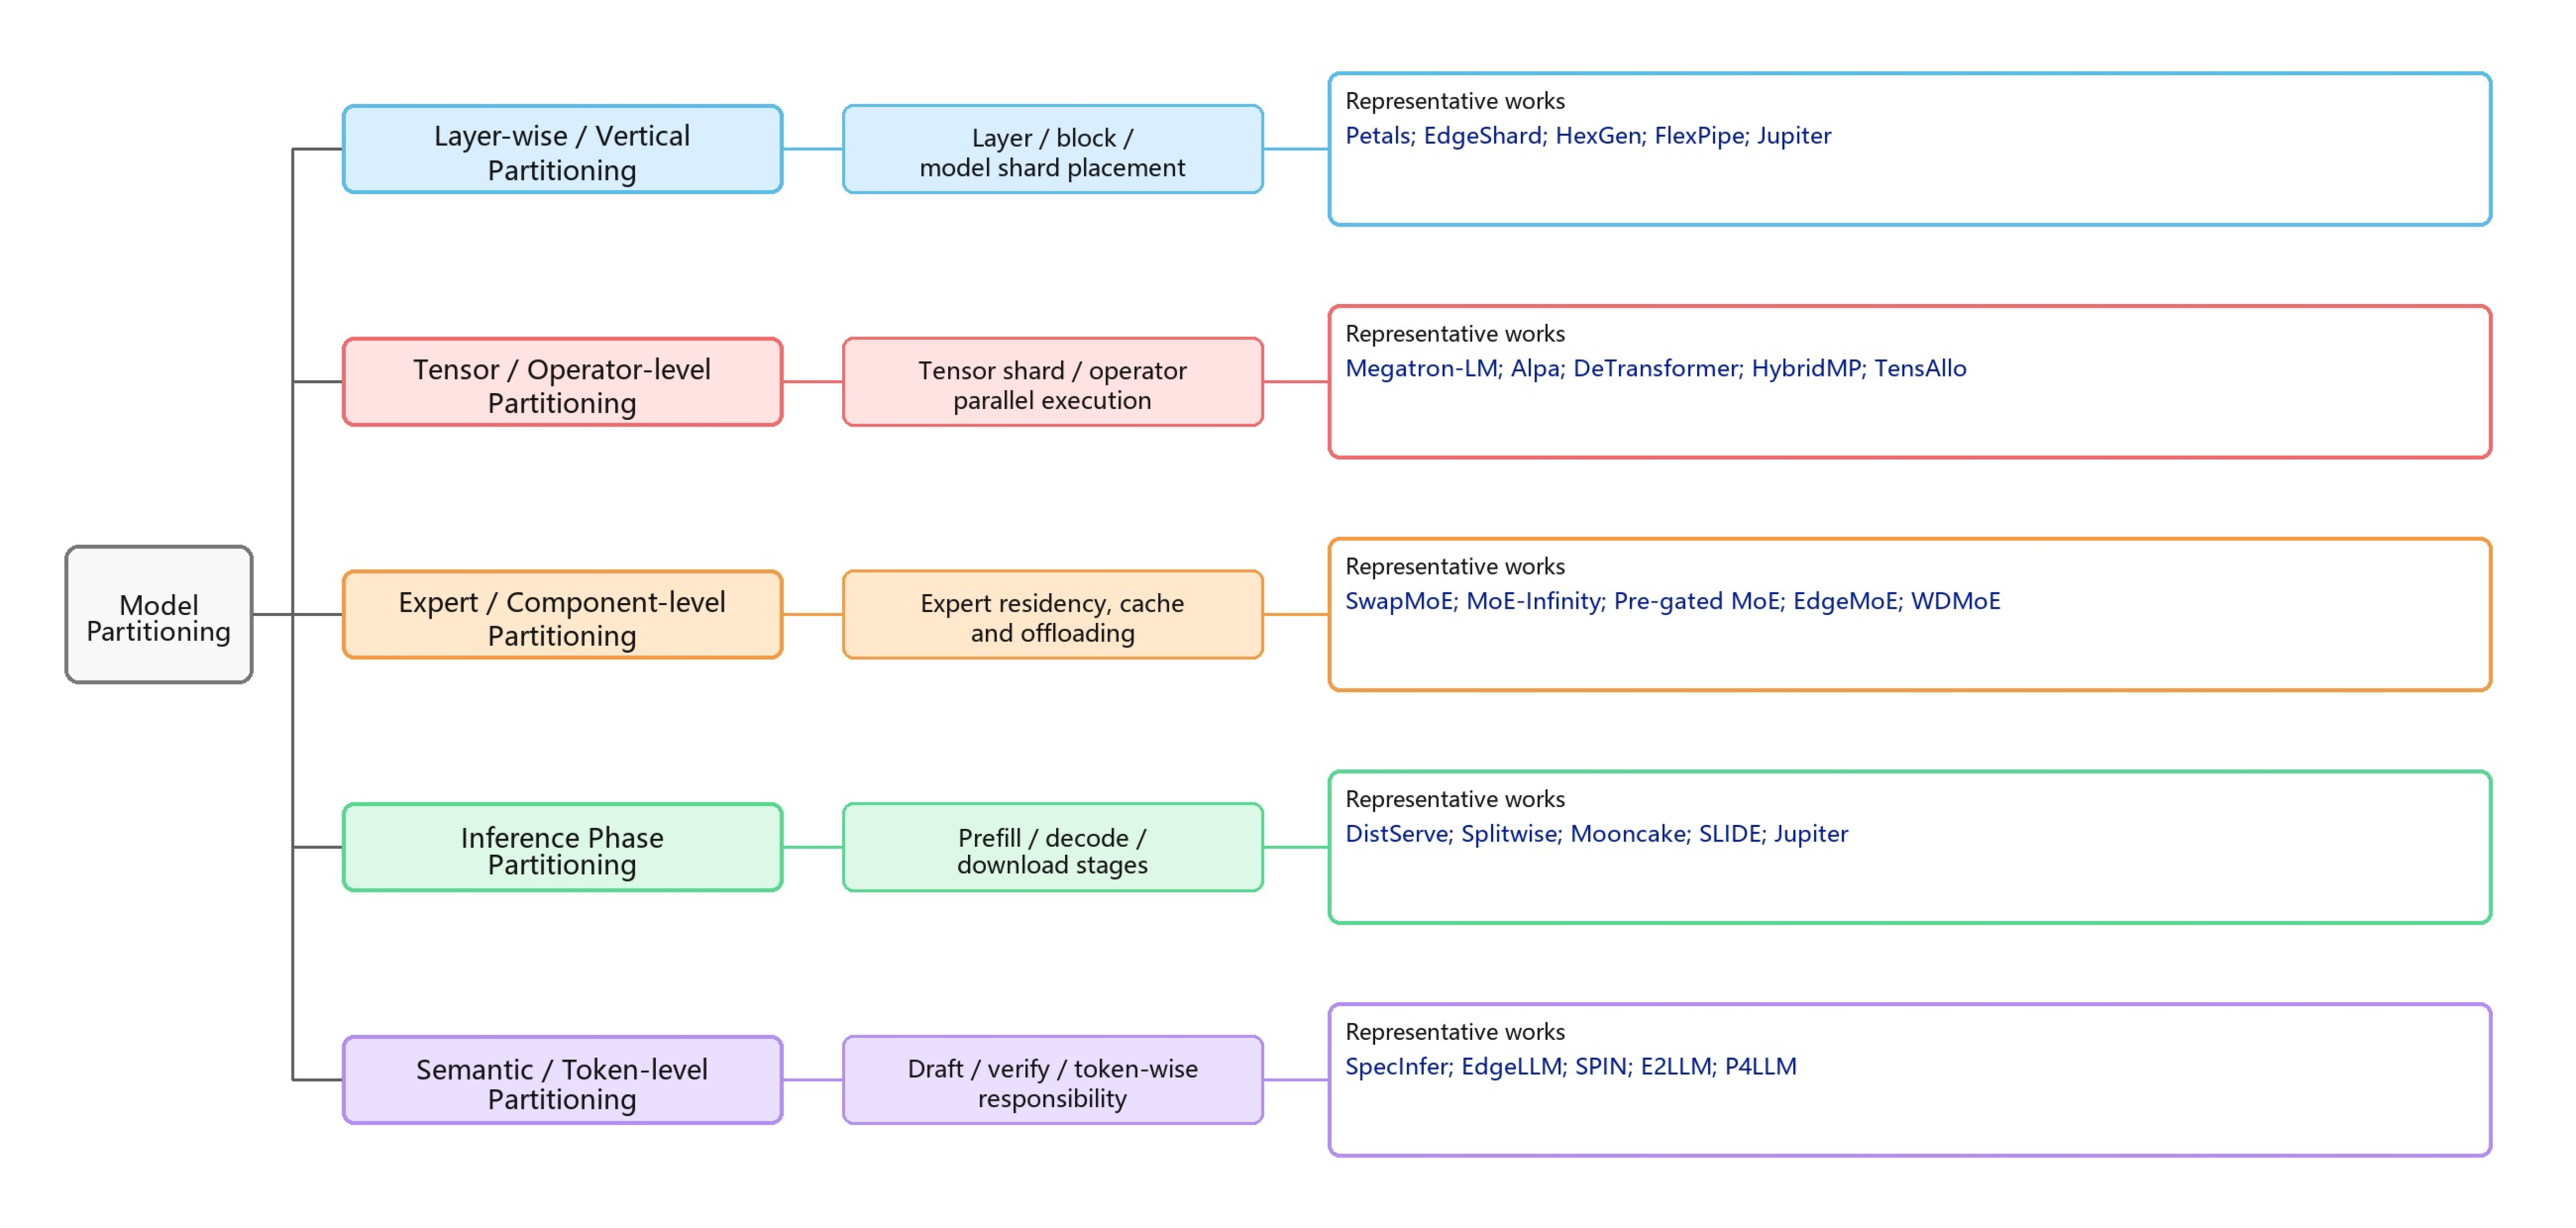
\includegraphics[width=\textwidth]{figures/ch4_model_partition_taxonomy.pdf}
\caption{\textbf{CEC 下资源自适应模型切分部署方法的分类树}}
\label{fig:cec-model-partition-taxonomy}
\end{figure}


\phantomsection
\subsection*{4.1 Layer-wise / Vertical Partitioning}
\addcontentsline{toc}{subsection}{4.1 Layer-wise / Vertical Partitioning}
层级切分是最接近传统意义上“模型分割”的一类方法。它把 Transformer 视为由多个顺序 block 组成的计算链，在 layer 或 block 边界上拆分模型，并将不同模型段放置到端侧、边缘或云端节点执行。对于无法完整加载模型权重、activation 和运行时状态的端侧或边缘设备，层级切分提供了一种直接的扩展方式：单个节点不再承担完整模型，而是多个节点共同完成同一次 forward。Petals 展示去中心化 block 放置 \cite{borzunov2023petals}，EdgeShard 面向边缘 shard placement \cite{zhang2024edgeshard}，HexGen 讨论异构生成式推理 \cite{jiang2023hexgen}，FlexPipe 则关注 serverless 集群中的 pipeline 重构 \cite{lin2026flexpipe}；这些工作共同验证了沿深度方向拆分模型的价值。

为了把这种“沿深度方向展开”的执行方式与普通请求路由区分开，可以参考图~\ref{fig:ch4-layerwise-partitioning}。
\begin{figure}[!htbp]
\centering
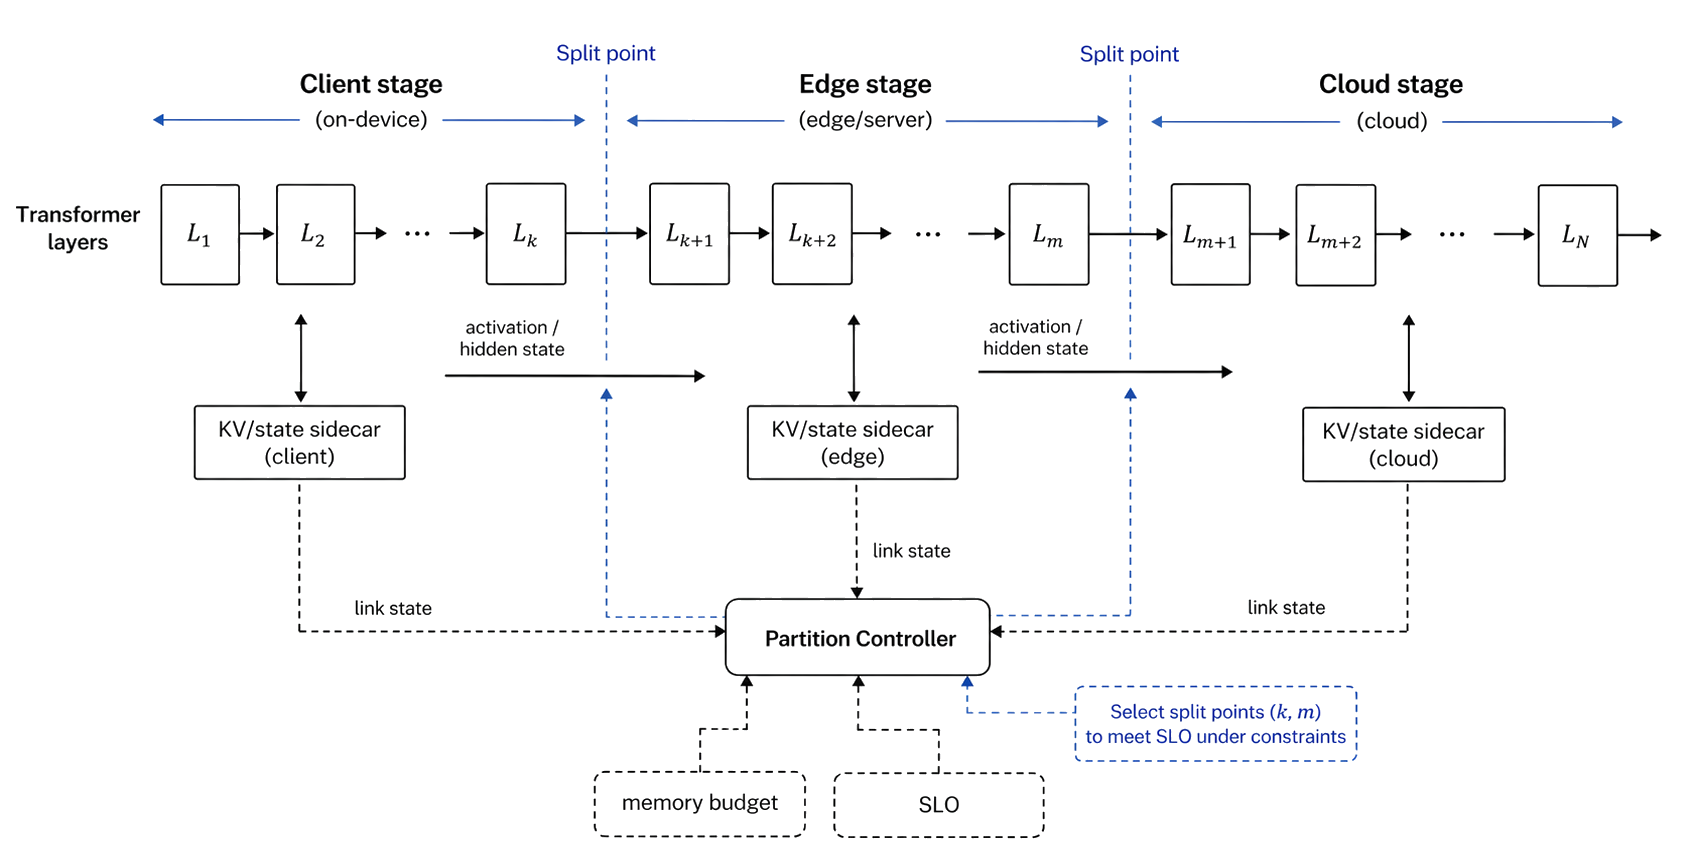
\includegraphics[width=\textwidth]{figures/ch4_2_layerwise_vertical_partitioning.png}
\caption{\textbf{Layer-wise / Vertical Partitioning 机制示意图}}
\label{fig:ch4-layerwise-partitioning}
\end{figure}
示意图中横向排列的 Transformer layers 表示同一个模型在深度方向上的执行链，虚线边界表示可选 split point。Client、Edge 和 Cloud 并不对应固定层数，而是代表不同资源层级；层间箭头表示 activation 或 hidden state 的跨节点传输，KV/state sidecar 表示推理过程中需要伴随模型段管理的运行时状态。Partition Controller 根据链路状态、显存余量、节点负载和 SLO 选择 layer placement、pipeline stage 与 fallback path。因此，层级切分的关键不是平均切开模型，而是在计算节省和跨节点状态传输之间动态权衡。

这一类方法的核心不是“把模型平均切开”，而是寻找合适的 split point 和 placement。切分点靠前，可以减轻端侧计算和内存压力，但会更早产生跨节点 hidden state 或 activation 传输；切分点靠后，可以降低网络依赖，却要求端侧执行更多 layer。对于长上下文请求，activation 规模和 KV 状态增长会进一步放大通信成本；对于短请求，通信启动时延可能抵消计算节省。因此，层级切分通常需要同时估计每层计算量、activation 大小、显存占用、链路带宽、RTT、节点负载和功耗约束。

CEC 环境使层级切分比云端 pipeline parallelism 更难。数据中心内的互联带宽相对稳定，而端-边、边-边、边-云链路可能受到无线抖动、跨域转发和拥塞影响。一个在静态 profiling 中最优的切点，到了移动用户、突发请求或边缘节点过载时可能迅速失效。因此，资源自适应的层级切分往往需要三类能力：离线阶段建立 layer-level profile，在线阶段根据节点和链路状态选择切点，运行时阶段在负载变化时进行有限频率的重配置。GPipe 体现了 pipeline parallelism 在稳定集群中的基本价值 \cite{huang2019gpipe}，Megatron-LM 展示了大模型 tensor parallelism 的基础路线 \cite{narayanan2021efficient}，Alpa 则进一步自动化 inter-operator 与 intra-operator parallelism \cite{zheng2022alpa}。CEC 需要在这些并行思想之上继续纳入异构链路和在线状态。

这类方法还要处理流水线稳定性。切分后，每个模型段的执行时间如果差异过大，较慢节点会成为 pipeline bottleneck；中间节点失败或链路恶化时，后续 layer 是否迁移、是否重新选择切点、是否回退到云端完整执行，都会影响服务连续性。对于 CEC LLM 推理，层级切分不能只作为部署算法讨论，还必须和 admission control、状态管理和异常回退衔接。

总体来看，层级切分适合模型容量和单节点部署能力不足的场景，尤其适用于模型段执行时间差异明显、节点间链路相对稳定、跨节点 activation 可控的系统。它的主要风险在于切分收益被网络传输和流水线等待抵消。因此，CEC 中的层级切分更适合采用“少量稳定切点 + 在线代价修正”的方式，而不是频繁改变模型执行拓扑。

这里的“少量稳定切点”并不意味着静态平均切分，而是指将在线搜索限制在经过 profiling 验证、可部署且不会 OOM 的候选切点集合内，避免运行时任意切分造成模型重加载和状态迁移震荡。
\phantomsection
\subsection*{4.2 Tensor / Operator-level Partitioning}
\addcontentsline{toc}{subsection}{4.2 Tensor / Operator-level Partitioning}
当层级切分仍不足以缓解单层计算和显存压力时，系统需要进入更细粒度的张量/算子级切分。LLM 的每一层内部包含 attention、QKV projection、MLP、归一化和通信同步等多个计算单元，其中 attention head、矩阵乘和中间 activation 都可能成为单设备瓶颈。张量/算子级切分不再以完整 block 为边界，而是在同一层内部拆分 tensor、head、矩阵维度或 operator 执行路径。Megatron-LM 和 Alpa 代表了数据中心大模型中 tensor / intra-operator parallelism 的基础路线 \cite{narayanan2021efficient}, \cite{zheng2022alpa}；DeTransformer 通过结构协同设计降低分布式推理通信 \cite{du2024co}，Galaxy+ 采用混合模型并行组织边缘 Transformer 推理 \cite{ye2025resource}，TensAllo 则把异构边缘设备选择和 tensor allocation 纳入部署决策 \cite{zhang2025tensallo}。

层内拆分的系统关系可以用图~\ref{fig:ch4-tensor-operator-partitioning} 概括，它突出的是同一 Transformer 层内部的并行和同步，而不是层与层之间的顺序切点。
\begin{figure}[!htbp]
\centering
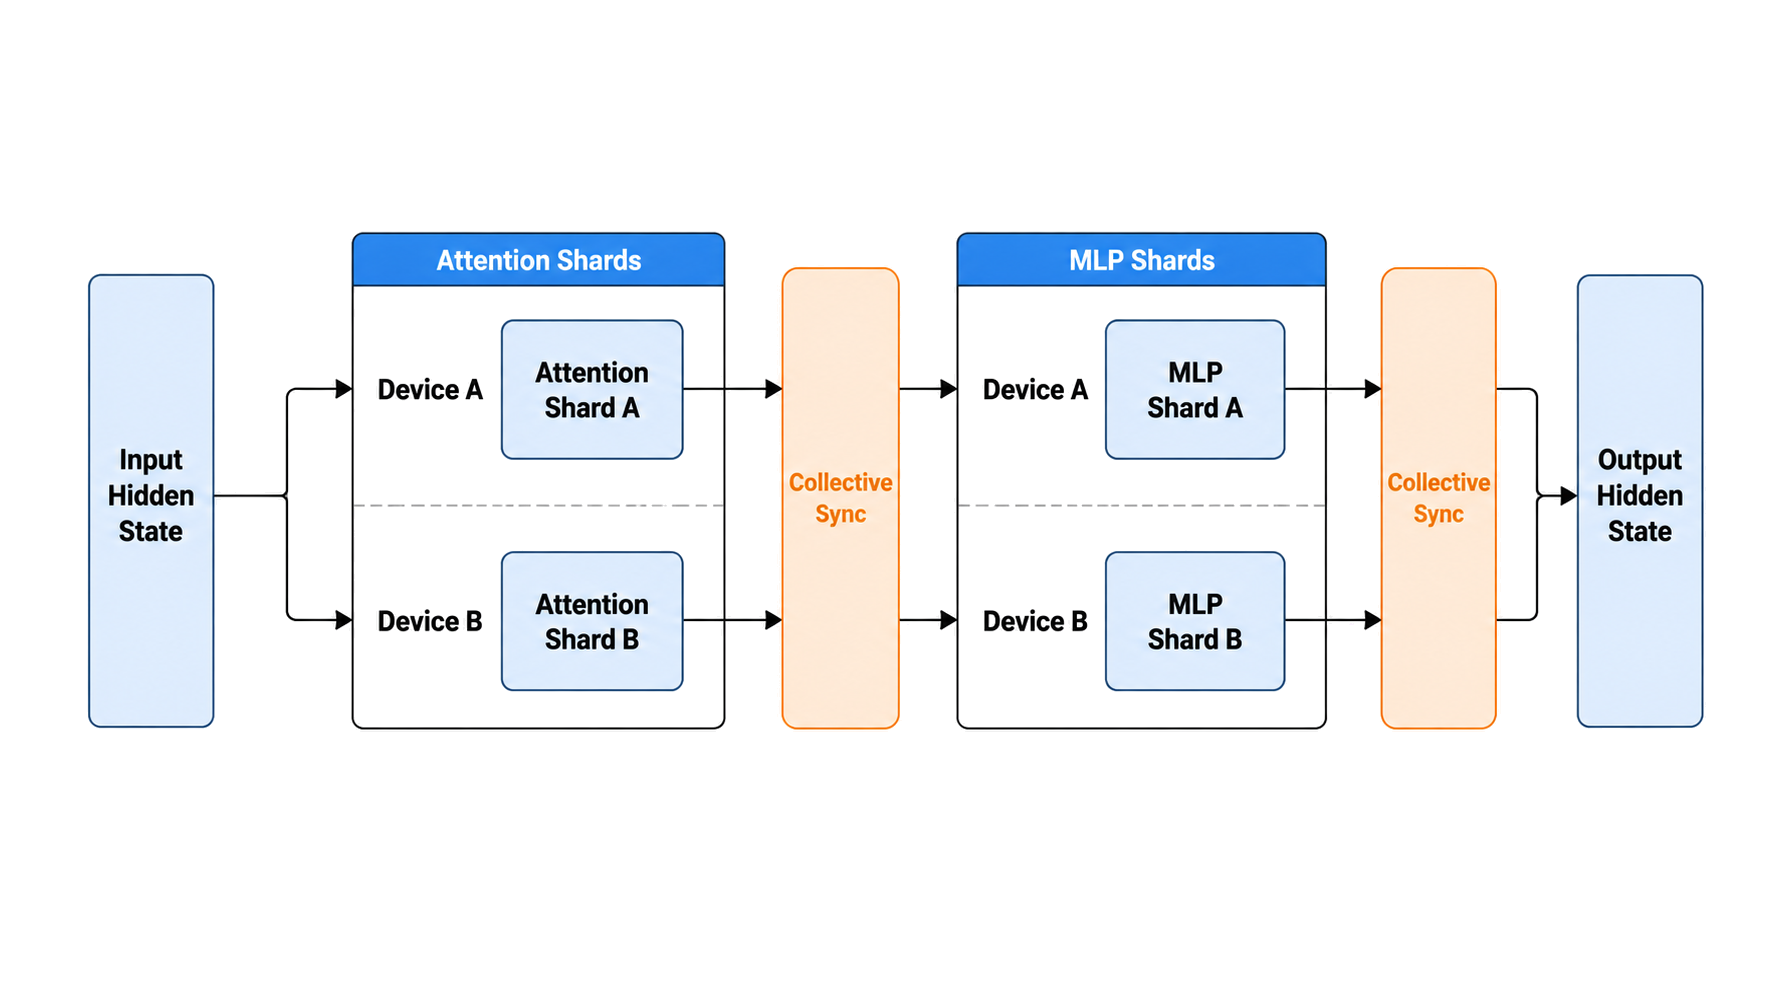
\includegraphics[width=\textwidth]{figures/ch4_3_tensor_operator_partitioning.png}
\caption{\textbf{Tensor / Operator-level Partitioning 机制示意图}}
\label{fig:ch4-tensor-operator-partitioning}
\end{figure}
图中没有展开每个 GEMM 或 attention kernel 的细节，而是保留张量/算子级切分最关键的执行关系：左侧是单个 Transformer layer，中间的 Partition Planner 根据 layer profile、硬件拓扑、显存预算和 SLO 判断是否需要层内并行；右侧的 Device Group 表示同一层被分配到多个 Ascend 设备上执行。Attention 部分可以按 head 或 QKV shard 拆分，MLP 部分可以按矩阵维度拆分；各设备得到局部结果后，再通过 all-gather、reduce-scatter 或 all-reduce 完成同步合并。这里的关键不是“多设备一定更快”，而是并行度增加后同步次数和链路依赖也会增加；在 CEC 中，边缘链路的带宽和抖动会直接决定水平切分是否有收益。

这类方法通常保持模型数学语义不变，改变的是层内计算如何分布到多个设备。它可以表现为 tensor parallelism、hybrid model parallelism、block parallelism、低通信 Transformer 结构或 structure-guided partitioning。与层级切分相比，它能更细地利用碎片化资源；与单机 kernel 优化相比，它必须显式处理跨设备通信、同步和拓扑选择。

本章将 Tensor / Operator-level Partitioning 视为比普通 kernel 优化更高一层的系统问题。若某项工作只优化单设备 GEMM/attention kernel，而不改变层内计算的跨设备分布，则不归入本类。

水平切分的核心矛盾是并行收益与通信惩罚。切得越细，单个设备承载的权重、activation 和中间矩阵越少，也更容易把多个弱设备组织起来；但 all-reduce、all-gather、reduce-scatter 或点对点传输会更频繁。切得越粗，通信开销下降，却可能重新遇到显存或算力瓶颈。数据中心可以依赖高速互联吸收一部分同步成本，CEC 中的边缘设备却往往只有普通以太网、无线链路或多跳边缘互联，过细的 tensor parallelism 很容易变成通信密集型执行。

因此，CEC 下的张量/算子级切分需要比云端并行更强的资源画像。调度器要知道哪些设备适合低比特 GEMM，哪些设备适合 attention，哪些设备只能承担较小 tensor shard；还要估计层内同步频率、通信 primitive 的代价和 batch size 对算子效率的影响。某些工作还通过模型结构 co-design 减少层内依赖，使模型天然更适合低通信分布式推理。这说明水平切分不是单纯调大 parallel degree，而是模型结构、设备选择和通信路径的联合设计。

张量/算子级切分适合单层计算或显存压力成为瓶颈的场景，但在 CEC 中不能简单照搬数据中心 tensor parallelism。边缘链路的带宽、抖动和同步延迟会直接决定并行收益是否存在。因此，这类方法应优先与低通信结构、异构设备选择和静态/动态 profiling 结合，并尽量避免让每个 token 都经过高频跨节点同步 \cite{zhang2025tensallo}, \cite{ye2025resource}, \cite{du2024co}。
\phantomsection
\subsection*{4.3 Expert / Component-level Partitioning}
\addcontentsline{toc}{subsection}{4.3 Expert / Component-level Partitioning}
专家/组件级切分主要面向 MoE 等具有显式内部组件选择机制的模型。与普通 dense Transformer 不同，MoE 模型通常在 FFN 部分包含大量 expert，而每个 token 只激活其中少数 expert。这个结构使模型天然具备“组件级可调度性”：系统不一定让所有 expert 同时常驻同一设备，而可以根据 expert 热度、token routing 分布、显存预算、链路状态和请求类型，决定哪些 expert 常驻、哪些按需换入、哪些放在边缘或云端节点上。SwapMoE 从 expert swapping 角度降低显存压力 \cite{kong2024swapmoe}，MoE-Infinity 利用 sparsity-aware expert cache 支撑个人设备上的 MoE 推理 \cite{xue2024moe}，Pre-gated MoE 通过提前 expert routing 协同系统调度 \cite{hwang2024pre}，EdgeMoE 面向移动端稀疏模型部署 \cite{yi2025edgemoe}，WDMoE 则讨论无线分布式 expert 放置和带宽分配 \cite{xue2025wdmoe}。这些工作共同说明，组件级切分已经成为 MoE 推理系统的重要组织方式。

MoE 场景下，组件驻留和 token routing 的关系更适合从图~\ref{fig:ch4-expert-component-partitioning} 这样的分层缓存视角理解。
\begin{figure}[!htbp]
\centering
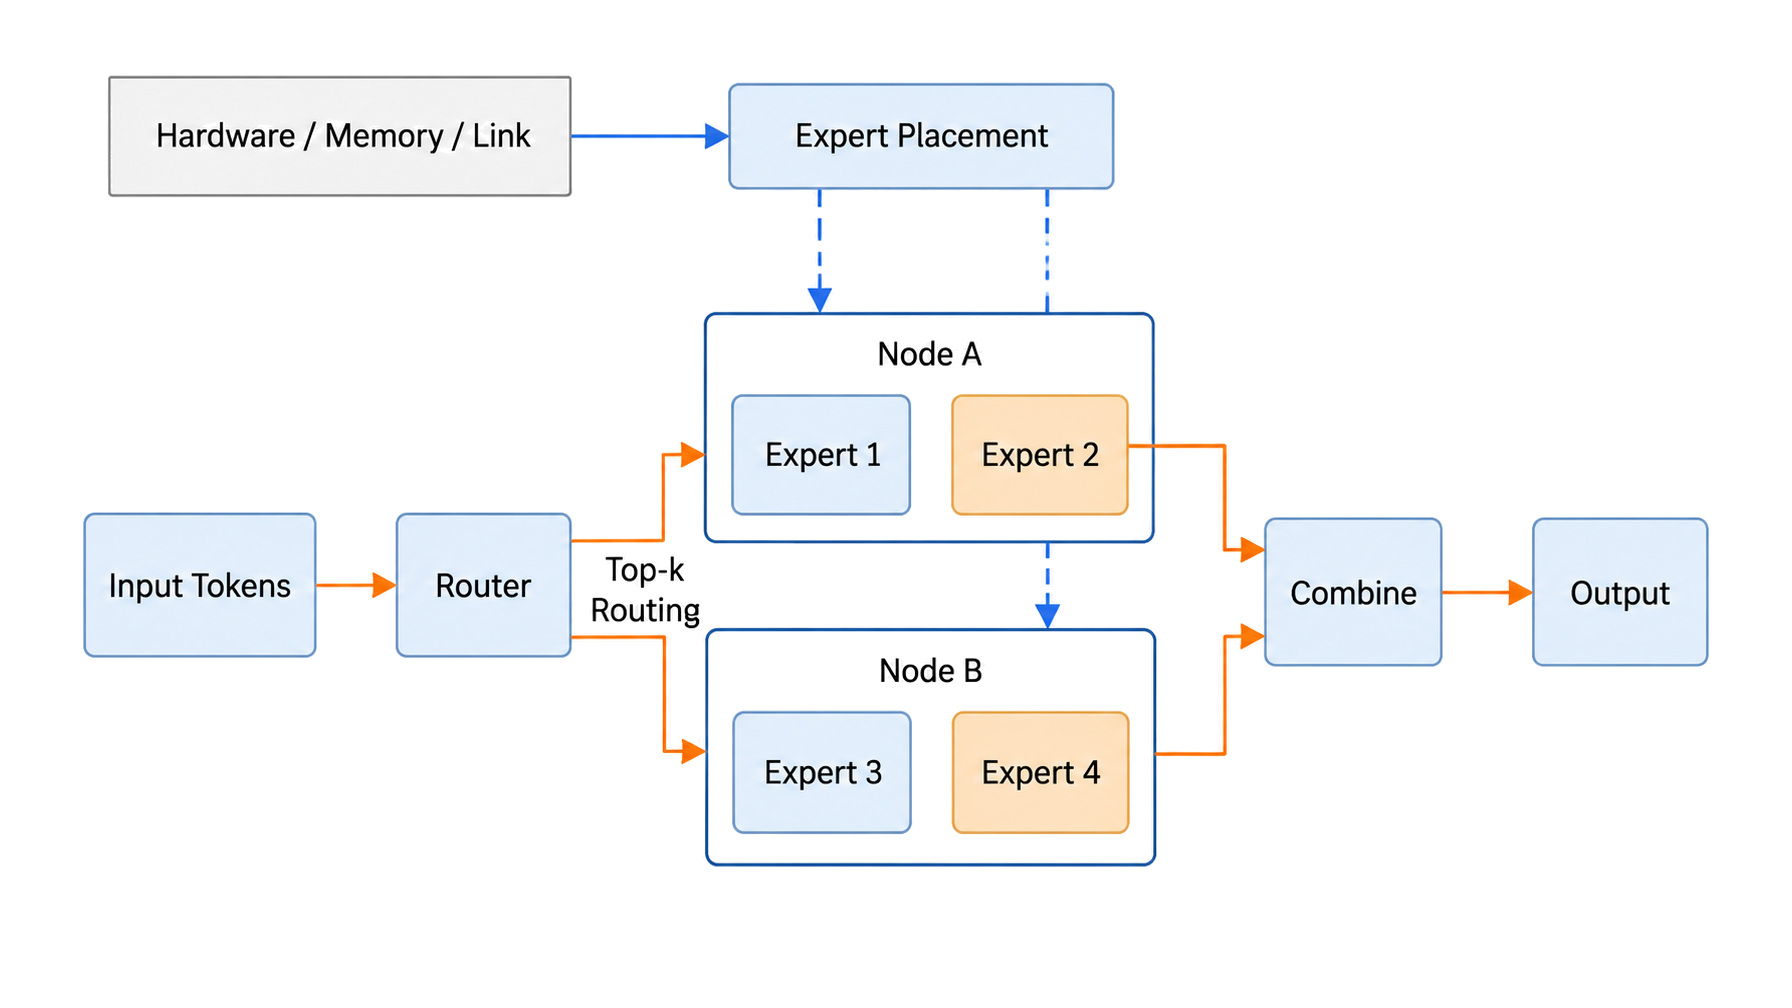
\includegraphics[width=0.86\textwidth]{figures/ch4_4_expert_component_partitioning.png}
\caption{\textbf{Expert / Component-level Partitioning 机制示意图}}
\label{fig:ch4-expert-component-partitioning}
\end{figure}
在这个机制中，MoE Router 为每个 token 选择 top-k experts，Expert Placement Policy 再根据 expert hotness、memory budget 和 link state 决定 expert 的驻留层级。热 expert 可以放入 Edge Expert Cache，次热 expert 放在 Regional Expert Pool，低频或完整 expert 集合保存在 Cloud / SSD Expert Store。箭头表示 token-expert 访问路径和 expert swap/prefetch 路径。组件级切分的收益来自稀疏激活和访问局部性，风险则来自 expert 预测错误后产生的远程访问或换入等待。

这一类方法之所以不直接并入张量/算子级切分，是因为它切的不是矩阵维度或 communication primitive，而是具有模型语义的组件单元。一个 expert 往往对应一组完整参数和计算路径，其是否被激活取决于 token-level routing；系统优化的对象也从“如何并行执行同一层矩阵”转向“如何管理大量稀疏激活组件的驻留、映射和调度”。因此，专家/组件级切分介于层内切分和语义/token 协同之间：它发生在模型内部组件层面，但收益取决于 token 分布和专家访问模式。

在 CEC 场景下，专家/组件级切分的价值在于降低大模型组件的常驻压力。端侧或接入边缘难以保存完整 MoE 模型，但可能保存高频 expert、局部业务相关 expert 或经过压缩的 expert cache；区域边缘可以维护更大的 expert pool；云端则保留完整 expert 集合并处理低频或复杂请求。系统需要在 expert 命中率、换入换出成本、跨节点 expert 访问时延和输出质量之间做权衡。如果 expert 热度预测准确，组件级切分可以减少显存占用并提高边缘可部署性；如果预测失误，频繁 swap 或远程访问 expert 会直接破坏 decode 时延。

专家/组件级切分的决策变量包括 expert residency、expert cache size、expert hotness prediction、token routing statistics、swap bandwidth、memory budget、fallback policy 和跨层级 expert placement。与层级切分相比，它更细粒度；与张量切分相比，它更依赖模型稀疏激活；与语义/token 级协同相比，它仍然保持同一个 MoE 模型内部的 expert 语义一致性，而不是把 draft、verify 或语义段分给不同模型完成。

总体来看，专家/组件级切分适合 MoE 模型、expert 热度具有局部性、边缘节点无法常驻完整 expert 集合的场景。它不应被简单理解为普通 request routing，因为请求仍在同一个 MoE 模型语义下执行；也不应被完全归入 token-level collaboration，因为系统主要调度的是 expert 组件而非生成职责。现有代表工作已经覆盖 expert swapping、fine-grained expert offloading、expert cache、pre-gating 和 wireless distributed experts 等不同角度；CEC 场景下仍然缺少把用户移动、区域业务热度、expert cache 迁移和无线带宽联合起来建模的工作 \cite{yu2026taming}, \cite{xue2025wdmoe}。

若目标模型是 dense LLM，本类方法一般不应作为模型切分部署的主路径；若目标模型或后续业务引入 MoE、专家模型或多 adapter 组件，本类才会成为核心部署问题。
\phantomsection
\subsection*{4.4 Inference Phase Partitioning}
\addcontentsline{toc}{subsection}{4.4 Inference Phase Partitioning}
LLM 推理不是单一形态的计算。Prefill 需要一次性处理完整 prompt，矩阵规模大、并行度高，通常更偏 compute-bound；decode 逐 token 生成，频繁访问 KV Cache，通常更偏 memory-bound 或 latency-bound；speculative decoding 中的 verification 又会形成目标模型批量校验；在无线边缘场景中，模型下载、加载和推理还可能同时出现在关键路径上。推理阶段切分正是利用这些阶段资源画像的差异，把不同阶段放到更合适的节点或资源池上执行。DistServe \cite{zhong2024distserve}、Splitwise \cite{patel2024splitwise} 和 Mooncake \cite{qin2025mooncake} 是 prefill/decode disaggregation 的代表；Jupiter 从边缘协作角度组织 prefill/decode 执行 \cite{ye2025jupiter}，E2LLM 从 Edge-IoT 结构化生成角度扩展阶段分工 \cite{feng20262}，SLIDE 则讨论无线边缘中的下载-推理重叠 \cite{qu2026slide}。

阶段级切分更适合放在推理流水线视角下理解，图~\ref{fig:ch4-inference-phase-partitioning} 给出了 prefill、decode、verification 与 KV/state handoff 的典型组织方式。
\begin{figure}[!htbp]
\centering
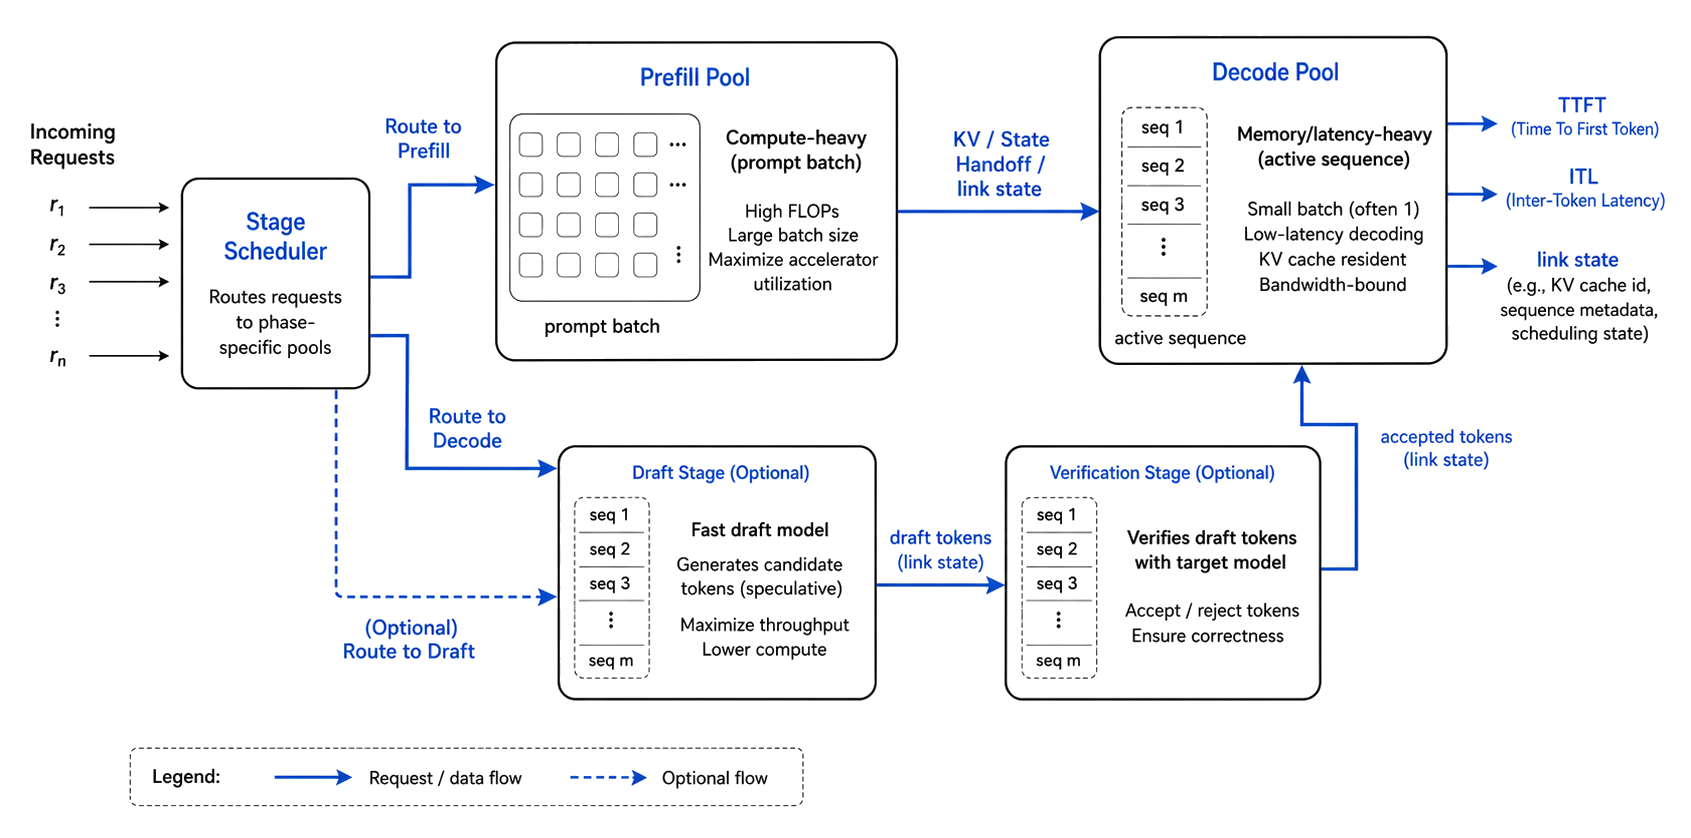
\includegraphics[width=\textwidth]{figures/ch4_5_inference_phase_partitioning.png}
\caption{\textbf{Inference Phase Partitioning 机制示意图}}
\label{fig:ch4-inference-phase-partitioning}
\end{figure}
这里的 Stage Scheduler 根据 prompt length、SLO、link state 和 KV locality 把请求送入不同阶段资源池。Prefill Pool 处理 compute-bound 的 prompt batch，Decode Pool 维护 memory/latency-bound 的 active sequence，KV / State Handoff 负责在阶段之间传递 KV blocks、metadata 和必要状态。若系统引入 verification 或 draft stage，它们也可以作为独立阶段被调度。阶段切分的核心收益来自资源画像匹配和阶段干扰隔离，核心代价则集中在 KV/state 传输与阶段队列协调。

最典型的形式是 prefill/decode disaggregation。长 prompt 的 prefill 可以放在算力更强、吞吐更高的区域边缘或云端实例，低时延 decode 则由更靠近用户的接入边缘承担。这样做可以减少长 prefill 对 decode 的阻塞，也能让不同硬件分别服务 compute-heavy 和 memory-heavy 阶段。进一步地，系统还可以把 draft generation 和 target verification 分开，或将模型下载与推理执行重叠，从而缩短冷启动和模型切换时延。

阶段切分的决策变量包括 prefill worker、decode worker、stage queue、pipeline boundary、KV transfer、verification placement、download/inference overlap 和阶段间同步机制。它的收益来自资源匹配和干扰隔离，但代价集中在状态交接。Prefill 和 decode 共享 KV Cache，draft 和 verify 共享候选 token 与概率校验状态，下载与推理重叠则会竞争网络、存储和内存带宽。换言之，阶段切分能否有效，取决于拆开之后能否低成本地把状态交给下一阶段 \cite{zhong2024distserve}, \cite{patel2024splitwise}, \cite{qin2025mooncake}。

在 CEC 中，阶段切分具有明显的场景价值。接入边缘适合承担低时延 decode，区域边缘适合聚合多个入口的 prefill-heavy 请求，云端适合长上下文、大模型 verification 或复杂推理。但这种分工不是无条件成立：如果 prefill 在云端完成后需要把大量 KV 传回边缘，链路抖动就会直接放大 TTFT 或后续 TPOT；如果边缘并发不足，独立 decode worker 可能无法形成有效 batch；如果用户移动导致入口切换，阶段边界还可能触发状态迁移。因此，阶段切分实际是在阶段资源匹配和状态连续性之间做权衡。

推理阶段切分适合 prefill/decode 负载差异明显、阶段队列规模足够、状态传输可控的场景。若请求很短、边缘并发很低或链路抖动大，复杂阶段拆分可能不如本地顺序执行稳定。因此，阶段切分必须和 KV 状态管理、链路预测、admission control 和回退策略一起设计；它不是独立的部署技巧，而是贯穿推理流水线的资源组织方式。

阶段切分与第五章的 Disaggregated Prefill-Decode Batching 视角不同。第四章关注 prefill/decode 是否跨实例或跨层级部署；第五章关注在已经分离的 prefill pool 与 decode pool 内部如何分别组批、排队和控制参数。
\phantomsection
\subsection*{4.5 Semantic / Token-level Partitioning}
\addcontentsline{toc}{subsection}{4.5 Semantic / Token-level Partitioning}
语义/token 级协同切分与前四类不同。它不一定把同一个模型的 layer、tensor 或 expert 组件拆开，而是把一次生成过程中的职责拆开：草稿由小模型产生，验证由大模型完成；长回答可以按语义段并行生成；隐私敏感 token 或 embedding 可以被单独 partition 和 perturbation。这里“切分”的对象是生成语义和 token 处理职责，而不是模型内部参数组件。SpecInfer 展示 token tree verification \cite{miao2024specinfer}，EdgeLLM 讨论端侧 speculative decoding \cite{xu2024edgellm}，SPIN 关注异构草稿模型选择 \cite{chen2025spin}，E2LLM 则展示语义段级并行生成 \cite{feng20262}。

生成职责级方法的结构可参考图~\ref{fig:ch4-semantic-token-partitioning}。它强调的不是参数如何分片，而是 draft、verify、refine 和 privacy filtering 等职责如何分配。
\begin{figure}[!htbp]
\centering
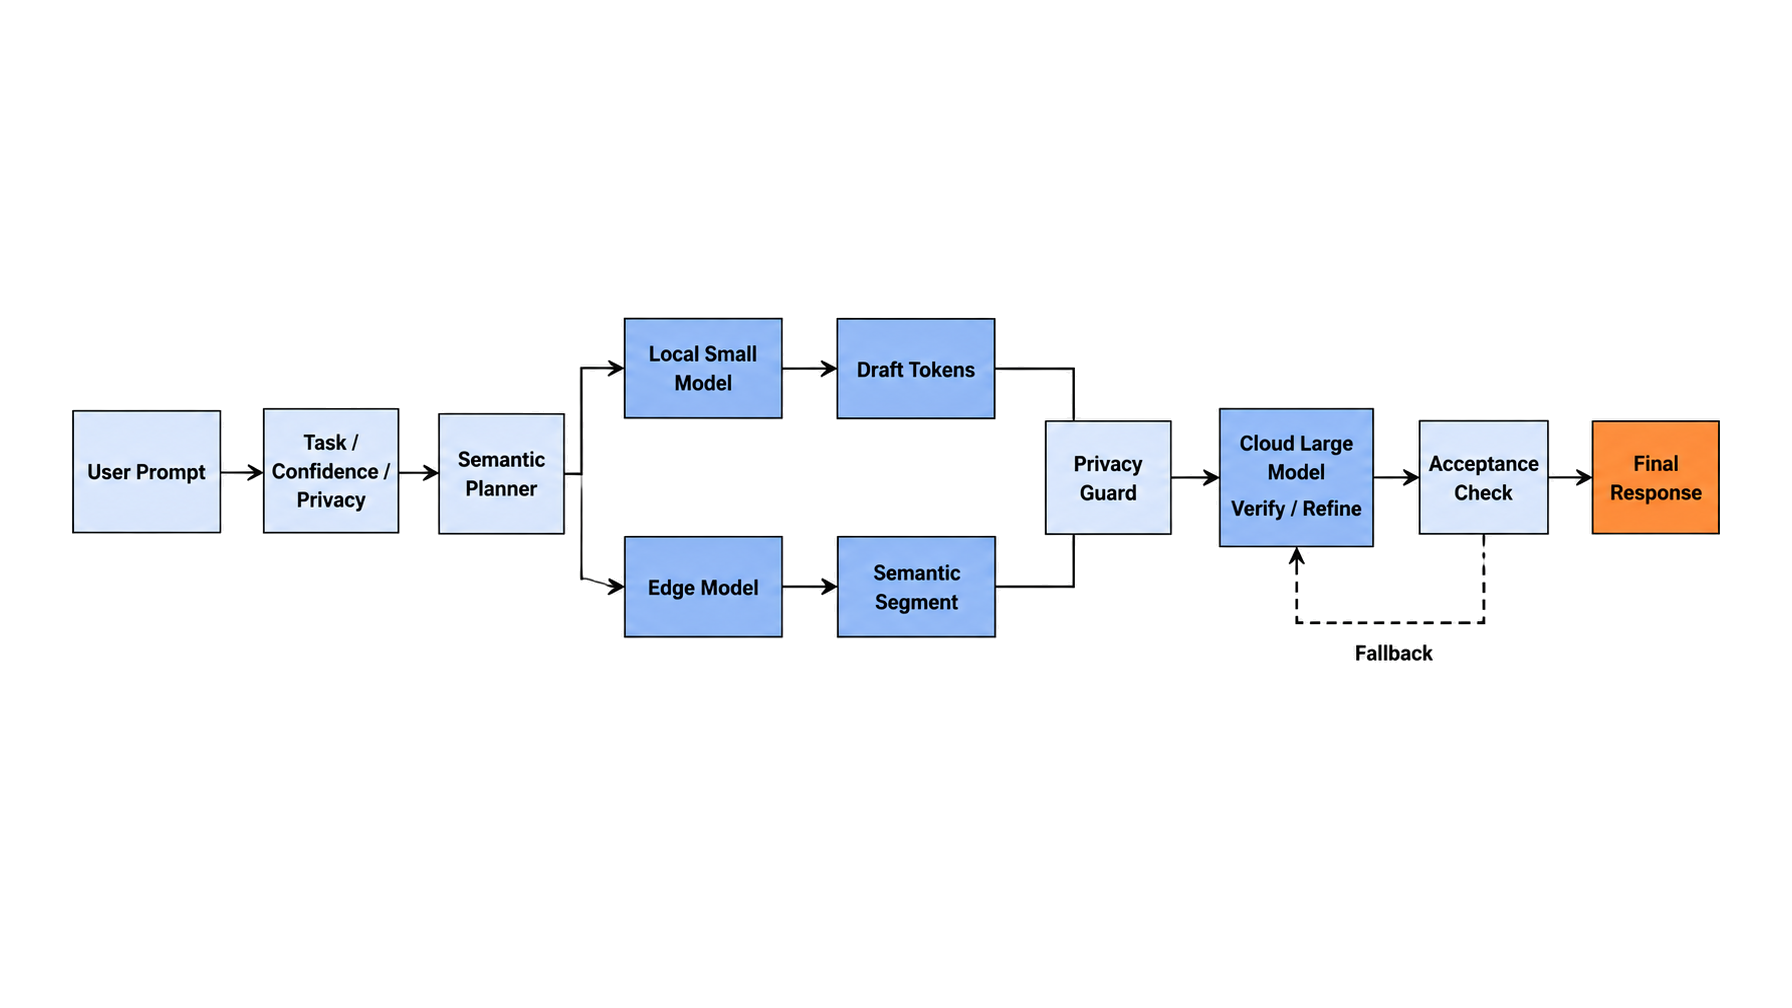
\includegraphics[width=\textwidth]{figures/ch4_6_semantic_token_partitioning.png}
\caption{\textbf{Semantic / Token-level Partitioning 机制示意图}}
\label{fig:ch4-semantic-token-partitioning}
\end{figure}
从系统路径看，Semantic Planner 根据 task type、confidence 和 privacy tag 判断每段生成职责交给哪个模块。Local Small Model 负责生成 draft tokens，Edge Model 可以承担部分 semantic segment generation，Privacy Guard 对敏感 token 做 partition 或 perturbation，Cloud Large Model 负责 verify/refine。Acceptance Check 决定草稿是否接受、是否回退到大模型重算。token/语义级方法的关键约束是质量一致性和错误回退，而不仅是加速。

这类方法的出发点，是自回归生成并不必然只能由一个模型连续完成。系统可以在端侧先生成 draft，再由边缘或云端目标模型 verify；可以先生成 response skeleton，再把不同语义段交给多个设备并行生成；也可以将隐私敏感 token 从普通 token 流中分离出来，采用额外扰动或分区策略。与层级切分和张量切分相比，它改变的是生成过程中的职责边界，而不是纯粹的模型拓扑 \cite{xu2024edgellm}, \cite{lu2026p4llm}。

语义/token 级协同的核心变量包括 draft length、acceptance rate、verification frequency、semantic segment boundary、token partition、privacy budget、fallback condition 和输出质量约束。它的收益通常来自减少大模型调用、并行化长回答生成或细粒度保护敏感信息；但风险也更直接地体现在输出质量上。draft 接受率过低会浪费验证计算，语义段边界选择不当会破坏上下文连贯性，过强的 token perturbation 可能损害语义一致性。

在 CEC 中，这类方法的意义在于把“端侧小模型、边缘模型、云端大模型协同”从请求级选择推进到生成级协作。端侧可以承担低成本 draft 或局部补全，边缘可完成常见语义验证或中等复杂度生成，云端大模型只在关键语义点介入。这样不仅有机会降低云端调用成本，也能改善交互时延和隐私边界。不过，这类方法对在线质量估计和回退机制要求最高，不能只依据资源指标判断收益。

语义/token 级协同切分适合端侧小模型可用、任务分布相对稳定、局部生成质量可被估计的场景。它的风险也最明显：低接受率、语义段不连贯或隐私扰动过强都会破坏质量。因此，这类方法需要和质量评估、置信度估计、安全回退以及外层服务策略联合设计，不能只用系统吞吐指标来评价。

本类中的 speculative decoding 工作不等价于“模型切分”本体；本章保留它们，是因为它们切分了 draft、verify、token tree 或语义段等生成职责，属于生成过程级的协同执行。
\phantomsection
\subsection*{4.6 面向华为验证环境的方案建议}
\addcontentsline{toc}{subsection}{4.6 面向华为验证环境的方案建议}

面向异构边缘验证环境，资源自适应模型切分部署首先要回答的是一个具体问题：在当前 Ascend 设备拓扑、显存水位、链路带宽和业务 SLA 下，模型应该在哪些 layer/block 之间切开，每一段应该放到哪个设备组上执行。因而推荐方案应以层级切分为主线，先让 Ascend GPU/NPU 推理栈支持连续 layer/block 形成跨卡、跨节点 stage 的执行，再用动态规划生成 stage boundary 和 stage placement 策略。TP、PP、EP、DP replica、KV migration 或 PD 分离等能力不作为人工挑选的“大方法”，而是在 runtime 支持且资源检查通过时被用于降低某个 stage 的显存、时延或吞吐压力。该思路与 EdgeShard 将 model shard placement 转化为动态规划搜索的思想一致，但落点更贴近华为验证环境中的层级切分执行能力建设 \cite{zhang2024edgeshard}。

具体而言，系统先采集三类画像。第一是设备资源与能力画像：根据硬件环境信息构建算力拓扑图 \(H=(V,E)\)，节点记录 Ascend 卡或 vNPU 的可用算力、可用显存、显存带宽、当前负载和 runtime capability，边记录 HCCS、RDMA、以太网或跨主机链路的带宽、时延和抖动。第二是模型画像：解析 PyTorch 或 HuggingFace 模型的 config、权重和模块结构，得到 layer 数、每层参数量、activation 峰值、单 token KV Cache 增量、prefill/decode 计算量以及是否包含 MoE expert 或可拆分组件。第三是业务画像：从配置中读取目标并发、输入输出长度分布、P90/P99 TTFT、TPOT、E2E latency、SLA 等级、请求优先级以及是否允许 KV 迁移、PD 分离或降级回退。这些画像共同决定每个连续 layer 区间在不同设备组上的执行代价、显存风险和链路代价。

\begin{figure}[!htbp]
\centering
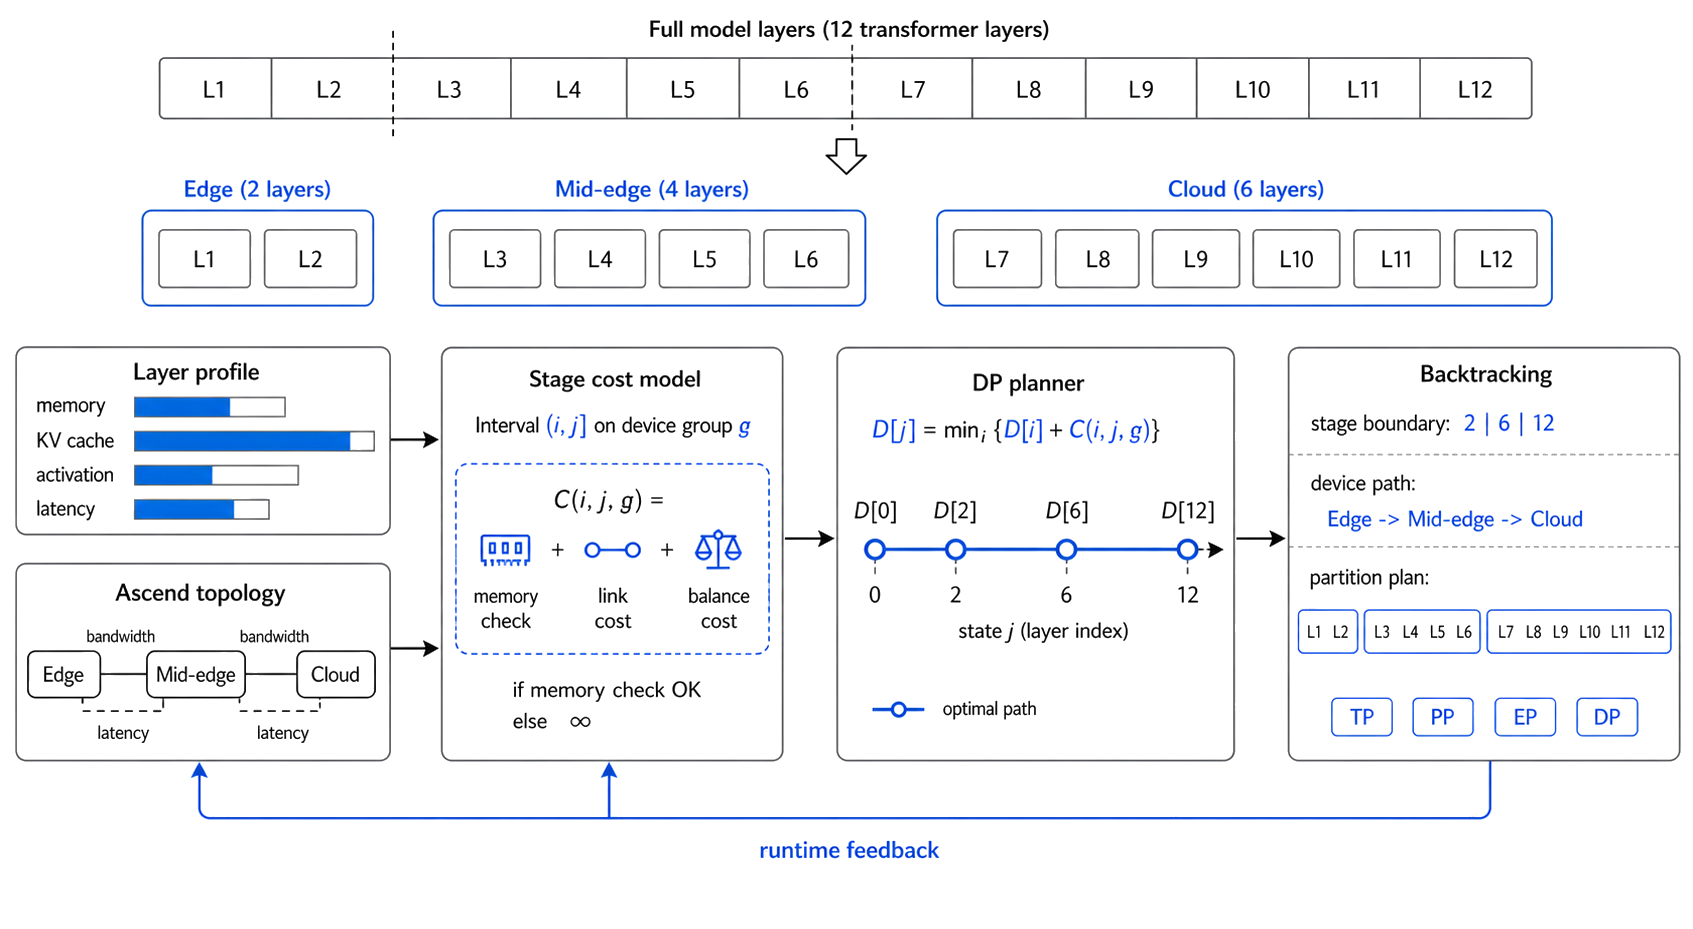
\includegraphics[width=\textwidth]{figures/ch4_dp_partition_architecture.png}
\caption{基于动态规划的层级切分部署策略生成流程}
\label{fig:ch4-dp-partition-architecture}
\end{figure}

如图~\ref{fig:ch4-dp-partition-architecture} 所示，层级切分策略由 layer profile、Ascend topology、stage cost model 和 DP planner 共同生成。为了避免把“切分方案”写成一个过于抽象的黑盒，第四章的决策变量可以明确写成
\[
x=\{K,\{l_k,g_k,e_k\}_{k=1}^{K}\}.
\]
其中，\(K\) 表示模型被切成多少个连续 stage；\(l_k\) 表示第 \(k\) 个 stage 的右边界，因此第 \(k\) 个 stage 覆盖 layer 区间 \((l_{k-1},l_k]\)，且 \(l_0=0,l_K=N\)；\(g_k\) 表示该 stage 放置到哪个 Ascend 设备组或节点组；\(e_k\) 表示该 stage 在当前 runtime 已支持范围内启用的执行能力，例如单设备执行、TP、PP+TP、EP、KV/offload 或阶段间状态传输。这样，第四章真正要决策的是“切在哪里、每段放哪里、每段用什么已支持执行能力”，而不是在几类并行方法之间做人工选择。

在论文建模上，可以把问题写成从安全可部署取值空间中选择低代价层级切分方案：
\[
\begin{array}{l}
x^\star=\arg\min\limits_{x \in \mathcal{X}_{\mathrm{safe}}} J(x),\\
J(x)=
w_t T(x)+w_c C(x)+w_m M(x)+w_b B(x)-w_g G(x).
\end{array}
\]
其中，\(\mathcal{X}_{\mathrm{safe}}\) 表示经过 runtime 支持检查、资源检查和 SLA 检查后的安全取值空间。\(T(x)\) 表示 TTFT、TPOT、E2E latency 和 pipeline bubble 等时延代价；\(C(x)\) 表示 activation/hidden state、KV 或 stage 交接带来的通信代价；\(M(x)\) 表示显存水位、runtime reserve 和 OOM 风险；\(B(x)\) 表示 stage 执行时间不均衡造成的流水线阻塞；\(G(x)\) 表示满足 SLA 的有效吞吐收益。这个目标函数不需要展开到每个 kernel，而是服务于验证环境中的部署决策：在不违反显存、链路和 SLA 约束的前提下，选择总代价更低、有效吞吐更高的层级切分方案。

这些决策变量的取值由系统自动生成。首先，规划器根据模型 layer 数和 layer profile 生成所有连续区间 \((i,j]\)，并用前缀和快速得到该区间的权重、activation 峰值、KV 增量和 prefill/decode 计算量。其次，根据 Ascend topology 生成可承载 stage 的设备组 \(g\)：单卡、同机多卡、跨节点设备组或端-边-云层级组合都要带有可用算力、可用显存、链路带宽和 RTT 信息。再次，runtime capability 决定 \(e_k\) 的取值：如果连续 layer stage 加载和跨设备 hidden state 传输可用，则允许层级 stage；如果 TP collective 可用且链路代价可接受，则允许该 stage 使用 TP；如果模型包含 MoE expert 且 runtime 支持 expert 驻留或换入，则允许 EP；如果 KV/offload 或阶段间状态传输已经被 runtime 支撑，也可以作为该 stage 的执行能力进入评估。未通过能力检查或资源检查的取值不会进入后续 DP 递推。

动态规划负责在这些可执行取值中生成最终层级切分策略。规划器先计算把连续区间 \((i,j]\) 放到设备组 \(g\) 上的 stage cost \(C(i,j,g)\)。这里的 \(C(i,j,g)\) 与图~\ref{fig:ch4-dp-partition-architecture} 中的写法一致，是一个经过能力检查后的综合代价：它内部会在 \(\mathcal{E}_{\mathrm{ok}}(i,j,g)\) 中选择可用执行方式 \(e\)，并同时计入执行时间、显存水位、同步/传输代价和 pipeline balance。图中 Edge、Mid-edge 和 Cloud 承载不同数量的连续 layer，表示 DP 输出的不是平均切分，而是受设备算力、显存和链路代价共同约束的不均匀层级分配。若某个区间超过显存预算、链路预算或 SLA 风险阈值，则该取值直接被丢弃。对保留下来的可执行取值，DP 按 layer 顺序递推，记录到达每个 block 位置的最小代价和前驱切点。若记 \(D[j]\) 为完成前 \(j\) 个 block 的最小综合代价，则可简化写成
\[
D[j]=
\min_{i<j,\ g \in \mathcal{G}_{\mathrm{ok}}}
\left\{
D[i]
+C(i,j,g)
\right\},
\]
其中，\(\mathcal{G}_{\mathrm{ok}}\) 表示当前可用于承载 stage 的设备组。若需要展开 \(C(i,j,g)\)，它可以理解为 profiling 得到的 stage 执行代价、由 activation/hidden state 大小和链路状态估计的传输代价、显存检查代价以及 pipeline balance 惩罚的加权和；\(\mathcal{E}_{\mathrm{ok}}(i,j,g)\) 表示该区间在该设备组上已通过能力和资源检查的执行方式。递推完成后，系统从最后一个 block 反向回溯前驱切点，得到完整的 stage boundary 序列；再把每个 stage 对应的设备组和执行能力写入部署计划。这样，DP 不是抽象地给出一个分数最低的方案，而是实际生成“第几层到第几层放在哪个设备组、每段采用什么已支持执行方式、失败时回退到哪条路径”的部署策略。

在线阶段不应频繁重切模型。系统可以在 P99 TTFT 超标、显存水位接近阈值、链路退化、请求长度分布明显变化或 runtime capability 发生变化时触发重规划；新方案只有在预估收益超过阈值且安全检查通过后才执行，否则保持当前部署或回退到固定 PP/TP、单节点部署、平均层级切分等基线。最终的分割策略可按“先层级、再并行、后扩展”的顺序组织：先用动态规划确定 layer-wise stage boundary、stage placement 和 pipeline balance；再在具体 stage 上按 runtime 支持情况启用 TP、EP、DP replica 或 KV 迁移等能力；最后把 PD disaggregation、KV Cache Pool、semantic/token-level collaboration 等作为扩展能力纳入验证。这样既避免把方案写成空泛的人工选择，也能把第四章落到可测试、可对比、可部署的华为验证路径上。
\phantomsection
\subsection*{4.7 小结}
\addcontentsline{toc}{subsection}{4.7 小结}

本章围绕“一次推理中首先被切分的对象”组织 CEC 下的资源自适应模型切分部署方法。Layer-wise / Vertical Partitioning 关注 layer、block 或 model shard 如何跨节点展开；Tensor / Operator-level Partitioning 关注同一层内部的 tensor、head、MLP 或通信 primitive 如何并行；Expert / Component-level Partitioning 关注 MoE expert 等组件如何驻留、换入和跨层级访问；Inference Phase Partitioning 关注 prefill、decode、verification、download 等阶段如何匹配异构资源；Semantic / Token-level Partitioning 则关注 draft、verify、semantic segment 或 token-wise responsibility 等生成职责如何拆分。这个分类强调的是系统优化对象，而不是论文使用的术语本身。

这五类方法之间存在明显的互补关系。层级切分和张量/算子级切分主要解决模型容量、显存和并行度问题；专家/组件级切分更适合 MoE 等具有稀疏激活结构的模型；阶段切分用于缓解 prefill 与 decode 之间的资源画像差异；语义/token 级切分则把协同推理推进到生成过程内部。CEC 场景下的关键不在于选择某一种“万能切分”，而在于根据模型结构、节点能力、链路状态、KV 位置、业务 SLA 和隐私边界选择合适的切分粒度。

从工程落地看，资源自适应切分不宜完全依赖一次性离线规划。离线 profiling 可以建立 layer cost、tensor cost、activation size、KV 增长和设备吞吐基线，并与 runtime capability 一起形成能力门控和代价估计；在线阶段仍需要根据负载、链路和请求长度修正这些代价。更稳妥的路线是“离线 profiling + 能力门控 + 事件触发动态规划重算 + 安全回退”：先判断 Ascend 推理栈在当前硬件拓扑上支持哪些切分和并行能力，再由动态规划搜索满足约束的低成本层级切分方案，最后通过收益阈值、冷却时间和回退路径避免频繁重配置。

结合本报告面向的验证环境，第四章的主线应放在以 Layer-wise / Vertical Partitioning 为基础的能力门控动态规划算法上。Layer-wise stage boundary、stage placement 和 pipeline balance 是主决策；tensor/operator-level、phase partitioning 和 expert/component-level 等方法不再作为人工挑选的“大方法”，而是映射到 vLLM-Ascend / MindIE 或 CANN 生态可支持、可压测、可回退的执行能力，例如 TP、PP、PP+TP、EP、layer sharding、context parallel、PD 分离、KV pool/offload 和 speculative decoding。Expert/component-level 与 semantic/token-level 方法适合作为扩展能力：前者用于 MoE 或组件化模型，后者适合端侧小模型可用且质量回退机制成熟的场景。这样既能覆盖研究前沿，也能将综述结论自然转化为可测试、可对比、可部署的算法方案。
